%%%%%%%%%%%%%%%%%%%%%%%%%%%%%%%%%%%%%%%%%%%%%%%%%%%%%%%%%%%%%%%%%%%%%%%%%%%%
%% Trim Size: 9.75in x 6.5in
%% Text Area: 8in (include Runningheads) x 5in
%% ws-ijfe.tex   :   8-11-05
%% Tex file to use with ws-ijm.cls written in Latex2E.
%% The content, structure, format and layout of this style file is the
%% property of World Scientific Publishing Co. Pte. Ltd.
%% Copyright 1995, 2002 by World Scientific Publishing Co.
%% All rights are reserved.
%%%%%%%%%%%%%%%%%%%%%%%%%%%%%%%%%%%%%%%%%%%%%%%%%%%%%%%%%%%%%%%%%%%%%%%%%%%%
%

\documentclass{ws-ijfe}

%%% standard pachages
\usepackage{ amsmath, amssymb, amsfonts, graphicx, epsfig, mathtools, epstopdf}
%%%
\usepackage[section]{placeins}
\usepackage{morefloats}
\usepackage{float}
%%%%%%%%%%%%%%%%%%%%%%%%%%%%%%%%%%%%
%%% pachage to write Indicator function as 'blackboard bold 1': \mathbbm{1}. Made a custom macro \1=\mathbbm{1}
\usepackage{bbm}
%%%%%%%%%%%%%%%%%%%%%%%%%%%%%%%%%%%%

%%%%%%%%%%%%%%%%%%%%%%%%%%%%%%%%%%%%
% This package gives the enumerate environment an optional argument
% which determines the style in which the counter is printed.
% http://www.ctex.org/documents/packages/table/enumerate.pdf
\usepackage{enumerate}
%%%%%%%%%%%%%%%%%%%%%%%%%%%%%%%%%%%%

% to use strike out \sout
\usepackage[normalem]{ulem}


%%%%%%%%%%%%%%%%%%%%%%%%%%%%%%%%%%%%
% To display the labels used in a tex file in the dvi file (for example, if a theorem is labelled with the \label command) use the package
%\usepackage{showkeys}
%This will display all labels (for example, in the case of a labelled theorem, the label of the theorem will occur in the margin of the dvi file.
%The command above by itself not only displays labels when they are first named but also when they are cited (or referenced). To disable this feature use the following %options with the showkeys package
%\usepackage[notref, notcite]{showkeys}
%%%%%%%%%%%%%%%%%%%%%%%%%%%%%%%%%%%%


%%%%%%%%%%%%%%%%%%%%%%%%%%%%%%%%%%%%
% It extends the functionality of all the LATEX cross-referencing commands (including the table of contents, bibliographies etc) to produce \special commands which a driver can turn into hypertext links; it also provides new commands to allow the user to write ad hoc hypertext links, including those to external documents and URLs.
% http://www.tug.org/applications/hyperref/manual.html
\usepackage[colorlinks=true, pdfstartview=FitV, linkcolor=blue,
            citecolor=blue, urlcolor=blue]{hyperref}
\usepackage[usenames]{color}
\definecolor{Red}{rgb}{0.7,0,0.1}
\definecolor{Green}{rgb}{0,0.7,0}
%%%%%%%%%%%%%%%%%%%%%%%%%%%%%%%%%%%%


%%%%%%%%%%%%%%%%%%%%%%%%%%%%%%%%%%%%
% It is a LaTeX package to act as generalized
% interface for standard and non-standard bibliographic style files (BibTeX).
% http://www.ctan.org/tex-archive/macros/latex/contrib/natbib/
%\usepackage[numbers]{natbib}
%\usepackage{natbib}
%%%%%%%%%%%%%%%%%%%%%%%%%%%%%%%%%%%%


%%%%%%%%%%%%%%%%%%%%%%%%%%%%%%%%%%%%
% a good looking way to format urls
% http://mirror.its.uidaho.edu/pub/tex-archive/help/Catalogue/entries/url.html
\usepackage{url}
% Define a new 'leo' style for the package that will use a smaller font.
\makeatletter\def\url@leostyle{%
 \@ifundefined{selectfont}{\def\UrlFont{\sf}}{\def\UrlFont{\scriptsize\ttfamily}}} \makeatother\urlstyle{leo}
%%%%%%%%%%%%%%%%%%%%%%%%%%%%%%%%%%%%%

% to add accents and comments
%\usepackage{ comment}


%% custom margins
%\def\baselinestretch{1.1}
\setlength{\voffset}{-0.5in}
\setlength{\hoffset}{-0.5in}
\setlength{\textheight}{8.5in}
\setlength{\textwidth}{6in}
%% or use geometry pacakge
%\usepackage[margin=1.1in, dvips, letterpaper]{geometry}


%%%%%%%%%%%%%%%%%%%%%%%%%%%%%%%%%%%%%
%\newtheorem{theorem}{Theorem}[section]
%\newtheorem{proposition}[theorem]{Proposition}
%\newtheorem{lemma}{Lemma}[section]
%\newtheorem{corollary}[theorem]{Corollary}

%\theoremstyle{definition}
%\newtheorem{definition}[theorem]{Definition}
%\newtheorem{definition}{Definition}[section]
%\newtheorem{example}[theorem]{Example}
%\newtheorem{example}{Example}[section]
%\theoremstyle{remark}
%\newtheorem{remark}[theorem]{Remark}

%\newtheoremstyle{dotless}{}{}{\itshape}{}{\bfseries}{}{ }{}
%\theoremstyle{dotless}
%\newtheorem{assumption}{Assumption}
%\renewcommand*{\theassumption}{(\Alph{assumption})}
%\numberwithin{equation}{section}
%\numberwithin{theorem}{section}
%\renewcommand{\labelitemi}{ {\small $\rhd$}}

%%%%%%%%%%%%%%%%%%%%%%%%%%%%%%%%%%%%%
%%% used for editing and making comments in color
% Example \ig{Remarks and Commets}
\newcommand{\ti}[1]{\textcolor[rgb]{0.00, 0.0, 0.98}{T\&I: #1} }
\newcommand{\ig}[1]{\textcolor[rgb]{1.00, 0.0, 0.98}{Ig: #1} }
\newcommand{\ii}[1]{\textcolor[rgb]{0.00, 0.60, 0.5}{II: #1} }
\newcommand{\rr}[1]{\textcolor[rgb]{0.00, 0.65, 0}{RR: #1} }
\newcommand{\trb}[1]{\textcolor[rgb]{1.00, 0.00, 0}{TRB: #1} }
%%%%%%%%%%%%%%%%%%%%%%%%%%%%%%%%%%%%%


%%%%%%%%%%%%%%%%%%%%%%%%%%%%%%%%%%%%%
%%%     Igor's macros
%% \mathcal Letters
\def\cA{\mathcal{A}}
\def\cB{\mathcal{B}}
\def\cC{\mathcal{C}}
\def\cD{\mathcal{D}}
\def\cE{\mathcal{E}}
\def\cF{\mathcal{F}}
\def\cG{\mathcal{G}}
\def\cH{\mathcal{H}}
\def\cI{\mathcal{I}}
\def\cJ{\mathcal{J}}
\def\cK{\mathcal{K}}
\def\cL{\mathcal{L}}
\def\cM{\mathcal{M}}
\def\cN{\mathcal{N}}
\def\cO{\mathcal{O}}
\def\cP{\mathcal{P}}
\def\cQ{\mathcal{Q}}
\def\cR{\mathcal{R}}
\def\cS{\mathcal{S}}
\def\cT{\mathcal{T}}
\def\cU{\mathcal{U}}
\def\cV{\mathcal{V}}
\def\cW{\mathcal{W}}
\def\cX{\mathcal{X}}
\def\cY{\mathcal{Y}}
\def\cZ{\mathcal{Z}}

%% \mathbb Letters
\def\bA{\mathbb{A}}
\def\bB{\mathbb{B}}
\def\bC{\mathbb{C}}
\def\bD{\mathbb{D}}
\def\bE{\mathbb{E}}
\def\bF{\mathbb{F}}
\def\bG{\mathbb{G}}
\def\bH{\mathbb{H}}
\def\bI{\mathbb{I}}
\def\bJ{\mathbb{J}}
\def\bK{\mathbb{K}}
\def\bL{\mathbb{L}}
\def\bM{\mathbb{M}}
\def\bN{\mathbb{N}}
\def\bO{\mathbb{O}}
\def\bP{\mathbb{P}}
\def\bQ{\mathbb{Q}}
\def\bR{\mathbb{R}}
\def\bS{\mathbb{S}}
\def\bT{\mathbb{T}}
\def\bU{\mathbb{U}}
\def\bV{\mathbb{V}}
\def\bW{\mathbb{W}}
\def\bX{\mathbb{X}}
\def\bY{\mathbb{Y}}
\def\bZ{\mathbb{Z}}

\def\I{\mathbb{I}}
\def\1{\mathbbm{1}}


\newcommand{\pd}[1]{\partial_{#1}}      % partial derivative
\newcommand{\indFn}[1]{1 \! \! 1_{#1}}  % indicator function
\newcommand{\set}[1]{\left\{#1\right\}} % set: {xyz}
\renewcommand{\mid}{\;|\;}              % mid bar with small spaces before and after: x | y
\newcommand{\Mid}{\;\Big | \;}          % big bar with small spaces before and after:

\DeclareMathOperator*{\esssup}{ess\,sup} % ess sup
\DeclareMathOperator*{\essinf}{ess\,inf} % ess inf
\DeclareMathOperator*{\argmin}{arg\,min} % argmin
\DeclareMathOperator*{\argmax}{arg\,max} % argmax
%%%%%%%%%%%%%%%%%%%%%%%%%%%%%%%%%%%%%

%%%%%% d for derivative
\def\d{\mathrm{d}} 

\usepackage{graphicx}
\usepackage{cleveref}
\graphicspath{ {graphs/} }
\newcommand\numberthis{\addtocounter{equation}{1}\tag{\theequation}}

\begin{document}

\markboth{Authors' Names}
{Instructions for Typesetting Camera-Ready Manuscripts}

%%%%%%%%%%%%%%%%%%%%% Publisher's Area please ignore %%%%%%%%%%%%%%
\catchline{}{}{}{}{}
%%%%%%%%%%%%%%%%%%%%%%%%%%%%%%%%%%%%%%%%%%%%%%%%%%%%%%%%%%%%%%%%%%%

\title{Computing Option Prices Based on Heston Model to a Specified Tolerance\footnote{Typeset title in
10~pt Times Roman uppercase and boldface. Please write
down in pencil a short title to be used as the running head.}}

\author{Xiaoyang Zhao, Tianci Zhu and Fred J. Hickernell\footnote{Typeset names in 8~pt Times Roman, uppercase and lightface.  Use footnotes only to indicate if permanent and present addresses are different. Funding information should go in the Acknowledgement section.}}

\address{Full affiliations\footnote{Typeset
affiliation and mailing addresses in 8pt Times italic.} \\
,mailing addresses and telephone number}

\author{OTHER D. AUTHOR}

\address{Full affiliations \\
,mailing addresses and telephone number}

\maketitle

\begin{abstract}
Include a one-paragraph abstract of no more than 100 words. Do not include references, footnotes, or abbreviations in the abstract. Typeset the
abstract in 8 pt Times Roman with baselineskip of 10 pt, making
an indentation of $\frac14$ inch on the left and right margins.
Typeset similarly for keywords below.
\end{abstract}

\keywords{ Enclose with each manuscript, on a separate page, from three to five keywords. }

\section{Introduction}

We observed that in the financial market the volatility of asset prices may not be a constant. To have a more accurate pricing result, we need to implement an algorithm to simulate the volatility process. There are several well-known stochastic volatility models: the Hull-white model (1987), the Scott-Chesny model (1989), the Heston model (1993) and the SABR model (2002). We choose the Heston model as our approach since it is one of the most widely used stochastic volatility models. Upon solving the Heston model, the Quadratic Exponential (QE) scheme is used to simulate the volatility process and the Broadie-Kaya scheme is applied to the discretization of the asset price process.

However, the standard implementation gives inaccurate results when the volatility of the asset prices' volatility is set as zero. We identify this problem and fix it by a change of variables, which make it more accurate to calculate the Heston model. We compare the results with other simulation methods such as geometric Brownian motion and quasi-Monte Carlo, when setting the volatility of asset prices' volatility as zero, because in this case, the algorithm works like the one of asset price process with deterministic volatility. It shows that the new algorithm is accurate and fast. In addition, we implement the modified scheme in the Guaranteed Automatic Integration Library (GAIL) , which theoretically guarantees the result and stops algorithms automatically with user defined error tolerance .

The GAIL includes a suite of algorithms that applies the Monte Carlo methods for multidimensional integration and computation of means. The financial application module of GAIL is under construction, and our work is aimed to add algorithms of calculating stochastic volatility model in the asset path class.


The QE model was developed by \cite{Andersen2006}. It is a market standard simulation method for the Heston model. Its attractiveness lies in its efficiency. It relies on simple probability density functions and needs a moderate amount of storage. Depending on the value of the volatility, the QE scheme approximates its distribution using either Gaussian or exponential distribution. After getting the value of the volatility for each time step, we discretize the asset price process. As we know, the computation of Broadie-Kaya algorithm is time consuming, but it is bias-free by construction. We discretize its scheme to get the simulation of the dynamic of asset price process. The Broadie-Kaya scheme does not satisfy an equivalent discrete-time martingale condition. The martingale property can be attained by adjusting a certain term in the scheme.

The setup of the paper is as follows: we first introduce Heston model, QE scheme and the brief idea behind GAIL. Then, we explain our new algorithm and the improved algorithm using variance reduction techniques. At last, we show its performance in comparison with various widespread used schemes and with different variance reduction applications

\section{Options Modeled by the Heston Stochastic Volatility Model}
\subsection{Heston Model}
Heston model is defined as
 \begin{align}
    \d X & =\mu X\,\d t+\sqrt{V}X\,\d W_1\label{eq1}\\
    \d V &= \kappa (\theta-V)\,\d t +\nu\sqrt{V}\,\d W_2\label{eq2}
  \end{align}

 The first equation simulates the asset price process and the second equation gives the evolution of the volatility process. $X$ denotes the asset price. $V$ is the stochastic volatility process.  Two standard Brownian motions, $\d W_1$ and $\d W_2$, are set with a correlation constant $\rho$. $\mu$, $\kappa$, $\theta$, $\nu$ are constant parameters $\mu$ is the risk-free interest rate. $\kappa$ is the speed of mean reversion. $\theta$ is the value of the long-term variance. $\nu$ is the volatility of volatility.

%\begin{align*}
%\text{where }&\\
%   & X\text{ is the asset price process}\\
%   & V\text{ is the stochastic volatility process}\\
%   & \d W_1 \text{ and } \d W_2 \text{ are two standard Brownian motions which are correlated}\\
%   &\rho \text{ is the correlation,} \\
%   & \mu \text{ is the the risk-free interest rate,}\\%r \text{ and } d \text{ are respectively the continuously compounded risk-free interest rate and dividend yield,}  \\
%   & \kappa \text{ is the speed of mean reversion,} \\
%   & \theta \text{ is the value of the long-term variance,} \\
%   & \nu \text{ is the volatility of volatility.}
%\end{align*}

Applying the Ito's formula to Eq.\eqref{eq1}, an equivalent form to simulate the process of asset price is shown in Eq.\eqref{logX}.
\begin{equation}\label{logX}
  \d\ln(X)=(\mu-\frac{V}{2})\,\d t+\sqrt{V}\,\d W_1
\end{equation}

\subsection{Quadratic Exponential Scheme for Stochastic Volatility}
We applied the Quadratic Exponential Scheme illustrated in Andersen (2006) \cite{Andersen} to simulate the volatility process. Detailed steps are listed as follows:
\begin{enumerate}
\item Given $\hat{V}(t)$, compute $m$ and $s^2$ from following equations
\begin{align*}
  m &=\theta + (\hat{V}(t)-\theta)e^{-\kappa\Delta} \\
  s^2 &=\frac{\hat{V}(t)\nu^2 e^{-\kappa\Delta}}{\kappa}\bigg(1-e^{-\kappa\Delta}\bigg)+\frac{\theta\nu^2}{2\kappa}\bigg(1-e^{-\kappa\Delta}\bigg)^2
\end{align*}
\item Compute $\psi=s^2/m^2$\\
\item Draw a uniform random number $U_V$
\item If $\psi\leq\psi_c$:
\begin{enumerate}
\item Compute $a$ and $b$ from following equations
\begin{align*}
b^2=2\psi^{-1}-1+\sqrt{2\psi^{-1}}\sqrt{2\psi^{-1}-1}\geq 0, \qquad a =\frac{m}{1+b^2}.
\end{align*}
\item Compute $Z_V=\Phi^{-1}(U_V)$
\item Set $\hat{V}(t+\Delta)=a(b+Z_V)^2$
\end{enumerate}
\item Otherwise, if $\psi>\psi_c$
\begin{enumerate}
  \item Compute $\beta$ and $p$ according to equations
  \begin{align*}
    p & =\frac{\psi-1}{\psi+1}\in[0,1), \qquad%\\
    \beta =\frac{1-p}{m}=\frac{2}{m(\psi+1)}>0.
  \end{align*}
  \item set $\hat{V}(t+\Delta)=\Psi^{-1}(U_V;p,\beta)$
  \begin{equation*}
    \Psi(x) = \text{Pr}(\hat{V}(t+\Delta)\leq x) = p+(1-p)(1-e^{-\beta x}),\, x\geq 0
  \end{equation*}
  \[
  \Psi^{-1}(u)=\Psi^{-1}(u;p,\beta)=
  \begin{cases}
    0,\,&0\leq u \leq p,\\
    \beta^{-1}\ln(\frac{1-p}{1-u}),&p<u\leq1
  \end{cases}
  \]
\end{enumerate}
\end{enumerate}

\subsection{Broadie-Kaya Discretization Scheme for the Asset Prices}

We used the Broadie-Kaya scheme to simulate the asset price process. We give a brief derivation of this scheme here. Details are illustrated in \cite{Andersen2006}.

First we integrate the SDE for $V(t)$ to have a bias-free scheme,
\begin{equation*}
  V(t+\Delta) = V(t)+\int_{t}^{t+\Delta}\kappa(\theta-V(u))\,\d u +\nu\int_{t}^{t+\Delta}\sqrt{V(u)}\,\d W_V(u)
\end{equation*}
and it can be written as
\begin{equation}\label{dW_V}
\int_{t}^{t+\Delta}\sqrt{V(u)}\,\d W_V(u)=\nu^{-1}\bigg(V(t+\Delta)- V(t)-\int_{t}^{t+\Delta}\kappa(\theta-V(u))\,\d u\bigg)
\end{equation}
Recall Eq.\eqref{logX}, by Cholesky decomposition, we have
\begin{equation*}
 \d \ln X(t)=(\mu-\frac{1}{2}V(t))\,\d t +\sqrt{V(t)}\big(\rho\,\d W_V(t)+\sqrt{1-\rho^2}\,\d W(t)\big)
\end{equation*}
where $W$ is a Brownian motion independent of $W_V$.

Now we integrate the above equation,
\begin{equation*}
\begin{split}
  \ln X(t+\Delta)=&\ln X(t) +\mu\Delta-\frac{1}{2}\int_{t}^{t+\Delta}V(u)\,\d u +\rho\int_{t}^{t+\Delta}\sqrt{V(u)}\,\d W_V(u)\\ &+\sqrt{1-\rho^2}\int_{t}^{t+\Delta}\sqrt{V(u)}\,\d W(u)
\end{split}
\end{equation*}
Substituting Eq.\eqref{dW_V} into it, we get
\begin{equation}\label{lnX}
\begin{split}
   \ln X(t+\Delta)=&\ln X(t)+\mu\Delta+\frac{\rho}{\nu}(V(t+\Delta)-V(t)-\kappa\theta\Delta)+\bigg(\frac{\kappa\rho}{\nu}-\frac{1}{2}\bigg)\int_{t}^{t+\Delta}V(u)\,\d u\\
    &+\sqrt{1-\rho^2}\int_{t}^{t+\Delta}\sqrt{V(u)}\,\d W(u).
\end{split}
\end{equation}
We need to find appropriate approximation for the integrals in Eq.\eqref{lnX}. For now, we simply write
\begin{equation}\label{approx_du}
  \int_{t}^{t+\Delta}V(u)\,\d u \approx \Delta[\gamma_1 V(t)+\gamma_2 V(t+\Delta)]
\end{equation}
Conditioning on $V(t)$ and $\int_{t}^{t+\Delta}V(u)\,\d u$, the It$\hat{\text{o}}$ integral
$
  \int_{t}^{t+\Delta}\sqrt{V(u)}\,\d W(u)
$
is Gaussian with mean zero and variance $\int_{t}^{t+\Delta}V(u)\,\d u$. So, we write
\begin{equation*}
  \int_{t}^{t+\Delta}\sqrt{V(u)}\,\d W(u)\approx \Delta\sqrt{\gamma_1V(t)+\gamma_2V(t+\Delta)}\cdot Z
\end{equation*}
Therefore, we have the following discretiztion scheme
\begin{equation}\label{eq3}
  \text{ln}\hat{X}(t+\Delta)=\text{ln}\hat{X}(t)+K_0+K_1\hat{V}(t)+K_2\hat{V}(t+\Delta)+\sqrt{K_3\hat{V}(t)+K_4\hat{V}(t+\Delta)}\cdot Z
\end{equation}
where $Z$ is a standard Gaussian random variable, independent of $\hat{V}$, and $K_0,\dots,K_4$ are given by
\begin{align*}
  K_0&=-\frac{\rho\kappa\theta}{\nu}\Delta, &
  K_1&=\gamma_1\Delta\bigg(\frac{\kappa\rho}{\nu}-\frac{1}{2}\bigg)-\frac{\rho}{\nu}, &  K_2&=\gamma_2\Delta\bigg(\frac{\kappa\rho}{\nu}-\frac{1}{2}\bigg)+\frac{\rho}{\nu}, \\ K_3&=\gamma_1\Delta(1-\rho^2), & K_4&=\gamma_2\Delta(1-\rho^2).
\end{align*}
where $\gamma_1=\gamma_2=\frac{1}{2}$ in Anderson (2006).

\subsubsection{Implementation steps}
\textcolor[rgb]{1.00,0.00,0.00}{*Maybe delete implementation steps here and add those after our modification}\\
With given values of $\gamma_1$ and $\gamma_2$ and combined with the simulation scheme of $V$, the discretization scheme for ln$X$ can be generated in the following fashion:
\begin{enumerate}
  \item Given $\hat{V}(t)$, generate $\hat{V}(t+\Delta)$ using QE schemes
  \item Draw a uniform random number $U$, independent of all random numbers used for $\hat{V}(t+\Delta)$
  \item Set $Z=\Phi^{-1}(U)$
  \item Given ln$\hat{X}(t)$, $\hat{V}(t)$ and the value for $\hat{V}(t+\Delta)$ computed in Step 1, compute ln$\hat{X}(t+\Delta)$ from Eq.\eqref{eq3}
\end{enumerate}

%\subsubsection{Martingale correction}
Under the QE scheme, a martingale correction scheme is illustrated in Andersen (2006) as follows:
%\begin{equation*}
%E(\hat{X}(t+\Delta)|\hat{X}(t))=\hat{X}e^{K^*_0+(K_1+\frac{1}{2}K_3)\hat{V}(t)}E(e^{(K_2+\frac{1}{2}K_4)\hat{V}(t+\Delta)})=\hat{X}
%\end{equation*}

\begin{equation*}
  \text{ln}\hat{X}(t+\Delta)=\text{ln}\hat{X}(t)+K_0^*+K_1\hat{V}(t)+K_2\hat{V}(t+\Delta)+\sqrt{K_3\hat{V}(t)+K_4\hat{V}(t+\Delta)}\cdot Z
\end{equation*}
where
\[
  K_0^*=
  \begin{cases}
    -\frac{Ab^2a}{1-2Aa}+\frac{1}{2}\text{ln}(1-2Aa)-(K_1+\frac{1}{2}{K_3}){\hat{V}(t)},\,&\psi\leq\psi_c,\\
    -\text{ln}\bigg(\frac{\beta(1-p)}{\beta-A}\bigg)-(K_1+\frac{1}{2}{K_3}){\hat{V}(t)},&\psi>\psi_c
  \end{cases}
  \]
and $A=K_2+\frac{1}{2}K_4$.
\section{Overcoming Numerical Errors for Small Volatility of Volatility}
\subsection{Modification of QE scheme without martingale correction}
When $\nu$ equal or close to zero, the QE scheme we introduced above can be fragile. Our numerical results show that the option price given by QE scheme deviate from that calculated by exact sampling\footnote{Introduced by Broadie, M. and Kaya, O. (2006) for the Heston stochastic volatility model.They applied the numerical inversion of a cumulative distribution using the characteristic function. The estimator of an asset price generate using the sample stock price and variance from the exact distribution is unbiased. The scheme is computationally expensive, so we used it as benchmarks for result comparison.} and our modified scheme even further when the initial volatility $V_0$ not equals to long-term variance $\theta$. %So, we apply the change of variables technique to reduce the cancellation error.\\
\begin{figure}[h]
\centering
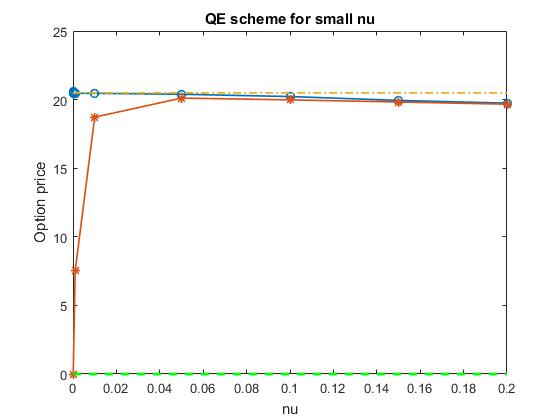
\includegraphics[width=0.55\textwidth]{FigureIn2_3_1}
\caption{European call option price calculated by QE scheme and our modified QE scheme. Initial price $=80$, strike $=100$, interest $=0$, $\kappa=1$, $\nu=0.5$, $\rho=-0.3$, $\theta=0.09$ and $V_0=0.36$. Small circles denote the price calculated by our modified QE scheme when the relative tolerance = 0.01 was met. The stars denote the price calculated by original QE scheme. The dot-dashed line denotes the option price calculated by Black-Scholes formula when $\nu=0$. The dashed line at the bottom denotes the option price given by QE scheme when $\nu=0$. }
\end{figure}
\begin{figure}[h]
\centering
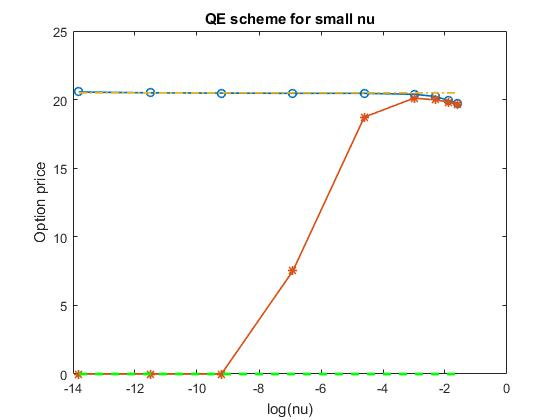
\includegraphics[width=0.55\textwidth]{FigureIn2_3_1_log}
\end{figure}

\subsubsection{Find more exact $\gamma_1$ and $\gamma_2$}
Recall Eq.\eqref{lnX}, the Broadie-Kaya scheme in integral form is written as
\begin{equation*}
\begin{split}
    \text{ln}X(t+\Delta)=&\text{ln}X(t)+\frac{\rho}{\nu}(V(t+\Delta)-V(t)-\kappa\theta\Delta)+\bigg(\frac{\kappa\rho}{\nu}-\frac{1}{2}\bigg)\int_{t}^{t+\Delta} V(u)du\\
     &+\sqrt{1-\rho^2}\int_{t}^{t+\Delta}\sqrt{V(u)}\,\d W(u).
\end{split}
\end{equation*}
We need to handle the time-integral of $V$. Rather than simply setting $\gamma_1=\gamma_2=\frac{1}{2}$, we want to find the exact value of $\gamma_1$ and $\gamma_2$ that make the following equation holds.\\
When $\nu=0$, the stochastic partial differential equation of $V$ (Eq.\eqref{eq2}) has a solution in form
\begin{equation}\label{V nu=0}
  V(t)=\theta + (V(0)-\theta)e^{-\kappa t}
\end{equation}
Denote $C=V(0)-\theta$,then $V(t)-\theta= Ce^{-\kappa t}$.\\
%\begin{equation}\label{V C}
%  V(t)-\theta= Ce^{-\kappa t}
%\end{equation}
We have
\begin{equation}\label{int V}
  \begin{split}
    \int_{t}^{t+\Delta}V(u)\,\d u&= \int_{t}^{t+\Delta}(V(u)-\theta)\,\d u+\theta\Delta\\
    &=\int_{t}^{t+\Delta}Ce^{-\kappa u}\,\d u +\theta\Delta\\
    &=\frac{-Ce^{-\kappa(t+\Delta)}+Ce^{-\kappa t}}{\kappa}+\theta\Delta\\
    %&=\frac{V(t)-\theta-V(t+\Delta)+\theta}{\kappa}+\theta\Delta.
  \end{split}
\end{equation}
We want find a expression of $\theta$ written in terms of $V(t)$ and $V(t+\Delta)$.\\
Set time to be $t+\Delta$ in Eq.\eqref{V nu=0} and multiply $e^{\kappa\Delta}$ on both sides, we have
%\begin{equation*}
%  V(t+\Delta)-\theta = Ce^{-\kappa(t+\Delta)}
%\end{equation*}
%Multiply $e^{\kappa\Delta}$ on both sides,
\begin{equation*}
  e^{\kappa\Delta}(V(t+\Delta)-\theta)=Ce^{-\kappa  t}
\end{equation*}
Combine with $V(t)-\theta= Ce^{-\kappa t}$, we have the expression of $\theta$ as
\begin{equation*}
%  \begin{split}
%    & e^{\kappa\Delta}V(t+\Delta)-V(t)+\theta(1-e^{\kappa\Delta})=0 \\
%    & \theta=\frac{V(t)-e^{\kappa\Delta}V(t+\Delta)}{1-e^{\kappa\Delta}}
%  \end{split}
\theta=\frac{V(t)-e^{\kappa\Delta}V(t+\Delta)}{1-e^{\kappa\Delta}}
\end{equation*}
Substitute the expression of $\theta$ into Eq.\eqref{int V}, we get
\begin{equation*}
  \begin{split}
    \int_{t}^{t+\Delta}V(u)\d u &= \frac{V(t)-V(t+\Delta)}{\kappa}+\Delta\frac{V(t)-e^{\kappa\Delta}V(t+\Delta)}{1-e^{\kappa\Delta}}  \\
    &=\frac{V(t)(1-e^{\kappa\Delta}+\kappa\Delta)-V(t+\Delta)(1-e^{\kappa\Delta}+\kappa\Delta e^{\kappa\Delta})}{\kappa(1-e^{\kappa\Delta})} \\
     %&=\Delta[\gamma_1 V(t)+\gamma_2 V(t+\Delta)]
     &=\Delta[\gamma V(t)+(1-\gamma) V(t+\Delta)]
  \end{split}
\end{equation*}
where
%\begin{align*}
%  \gamma_1 &= \frac{1-e^{\kappa\Delta}+\kappa\Delta}{\kappa\Delta(1-e^{\kappa\Delta})} &
%  \gamma_2 &= -\frac{1-e^{\kappa\Delta}+\kappa\Delta e^{\kappa\Delta}}{\kappa\Delta(1-e^{\kappa\Delta})}
%\end{align*}
%$\gamma_1 =
$\gamma = \frac{1-e^{\kappa\Delta}+\kappa\Delta}{\kappa\Delta(1-e^{\kappa\Delta})}$,
%$\gamma_2 = -\frac{1-e^{\kappa\Delta}+\kappa\Delta e^{\kappa\Delta}}{\kappa\Delta(1-e^{\kappa\Delta})}$.
%We know $\gamma_1\geq 0$ and $\gamma_2\geq 0$.\\
$\gamma\geq 0$.
As $\kappa\Delta\rightarrow 0$, $\gamma\rightarrow\frac{\frac{1}{2}(\kappa\Delta)^2}{\kappa\Delta}=\frac{1}{2} $.\\
%\begin{align*}
% \gamma_1 &\rightarrow\frac{\frac{1}{2}(\kappa\Delta)^2}{\kappa\Delta}=\frac{1}{2} \\
%  \gamma_2 &\rightarrow\frac{-(1+\kappa\Delta+\frac{1}{2}(\kappa\Delta)^2)(1-\kappa\Delta)+1}{\kappa\Delta(\kappa\Delta)}
%  \rightarrow\frac{-(1-(\kappa\Delta)^2)-\frac{1}{2}(\kappa\Delta)^2+\frac{1}{2}(\kappa\Delta)^3+1}{(\kappa\Delta)^2}\rightarrow\frac{1}{2}
%\end{align*}
When $\kappa\Delta$ goes to zero, our scheme just like the Euler scheme.\\
For $\nu\neq 0$, we approximate the integral $\int_{t}^{t+\Delta}V(u)\d u$ as follow:
\begin{equation*}
  \int_{t}^{t+\Delta}V(u)\d u = \Delta[\gamma V(t)+(1-\gamma) V(t+\Delta)] + O(\nu\Delta^{1.5}).
\end{equation*}
See the proof of the error order of this approximation in ~\ref{sec:AppendixA}.
\subsubsection{Change of variables}
We want to do change of variable of $s^2, m, \psi, b^{-2}, a, b, K_0,K_1,K_2, K_3,$ and $ K_4$ in a way that $\nu$ becomes multiplier rather than divisor.\\
For parameters in QE scheme, we do change of variables. As we see, new variables $\tilde{s}^2, \tilde{m}$ and $\tilde{\psi}$ are free of $\nu$.
%\begin{align*}
%s^2&=\nu^2\tilde{s}^2 & \tilde{s}^2 &=\frac{\hat{V}(t)e^{-\kappa\Delta}}{\kappa}\bigg(1-e^{-\kappa\Delta}\bigg)+\frac{\theta}{2\kappa}\bigg(1-e^{-\kappa\Delta}\bigg)^2, \\
%m&=\tilde{m} & \tilde{m} &=\Theta + \hat{V}(t)e^{-\kappa\Delta} \\
%  \psi&=\tilde{\psi}\nu^2, & \tilde{\psi}&=\bigg(\frac{\frac{\hat{V}(t)e^{-\kappa\Delta}}{\kappa}(1-e^{-\kappa\Delta})+\frac{\theta}{2\kappa}(1-e^{-\kappa\Delta})^2}{(\theta+(\hat{V}(t)-\theta)e^{-\kappa\Delta})^2}\bigg)\\
%  b^{-2}&=\nu^2\tilde{b}^{-2}, & \tilde{b}^{-2}&=\frac{\tilde{\psi}}{2\sqrt{1-\frac{\tilde{\psi}\nu^2}{2}}\bigg(1+\sqrt{1-\frac{\tilde{\psi}\nu^2}{2}}\bigg)} \\
%  a&=\tilde{a}\nu^2, & \tilde{a}&=\frac{m\tilde{b}^{-2}}{1+\nu^2\tilde{b}^{-2}}
%\end{align*}
\begin{align*}
s^2&=\nu^2\tilde{s}^2={\nu}^2\bigg(\frac{\hat{V}(t)e^{-\kappa\Delta}}{\kappa}\big(1-e^{-\kappa\Delta}\big)+\frac{\theta}{2\kappa}\big(1-e^{-\kappa\Delta}\big)^2\bigg),
\quad m=\tilde{m}=\theta + \hat{V}(t)e^{-\kappa\Delta}, \\
  \psi&=\nu^2\tilde{\psi}=\nu^2\bigg[\frac{\frac{\hat{V}(t)e^{-\kappa\Delta}}{\kappa}(1-e^{-\kappa\Delta})+\frac{\theta}{2\kappa}(1-e^{-\kappa\Delta})^2}{\big(\theta+(\hat{V}(t)-\theta)e^{-\kappa\Delta}\big)^2}\bigg],\\
b^{-2}&=\nu^2\tilde{b}^{-2}=\nu^2\frac{\tilde{\psi}}{2\sqrt{1-\frac{\tilde{\psi}\nu^2}{2}}\bigg(1+\sqrt{1-\frac{\tilde{\psi}\nu^2}{2}}\bigg)} ,\quad
a=\nu^2\tilde{a}=\nu^2\frac{m\tilde{b}^{-2}}{1+\nu^2\tilde{b}^{-2}}.
\end{align*}
Similarly, for parameters in Broadie-Kaya discretization scheme, we have
\begin{align*}
   K_0&=\frac{1}{\nu}\tilde{K}_0 =\frac{1}{\nu}(-\rho\kappa\theta\Delta),&   K_1&=\frac{1}{\nu}\tilde{K_1}=\frac{1}{\nu}\bigg[\rho(\kappa\gamma\Delta-1)-\frac{\nu\gamma\Delta}{2}\bigg],\\  K_2&=\frac{1}{\nu}\tilde{K_2}=\frac{1}{\nu}\bigg[\rho\big(\kappa(1-\gamma)\Delta-1\big)-\frac{\nu(1-\gamma)\Delta}{2}\bigg], &
   K_3&=\tilde{K}_3=\gamma\Delta(1-\rho^2),\\ K_4&=\tilde{K}_4=(1-\gamma)\Delta(1-\rho^2).
\end{align*}
%\subsubsection{Change of variables for calculating $\hat{X}$}
%For Eq.\eqref{eq2}, set $\nu=0$, we have
%\begin{equation*}
% \begin{split}
% \text{d}V(t)&=\kappa(\theta-V(t))\,\text{d}t\\
% V(T) &=\theta+(V(t)-\theta)e^{-\kappa(T-t)}
%\end{split}
%\end{equation*}
After doing change of variables, when $\nu$ goes to $0$, our new variables will be certain numbers rather than go to infinity.\\
Now we use new variables we defined to calculate $\hat{X}$. Recall Eq.\eqref{eq3}:
\begin{equation*}
  \text{ln}\hat{X}(t+\Delta)=\text{ln}\hat{X}(t)+K_0+K_1\hat{V}(t)+K_2\hat{V}(t+\Delta)+\sqrt{K_3\hat{V}(t)+K_4\hat{V}(t+\Delta)}\cdot Z
\end{equation*}
Observe the expression of parameters we discussed in section 2.3, the terms including $\frac{1}{\nu}$ will cause unstable of the scheme when $\nu$ is close or equal to zero. We want to define a new variable of stochastic volatility process $V$ in a way that there is no $\frac{1}{\nu}$ in our modified discretization scheme.\\
Write $\hat{V}(t+\Delta)$ in terms of new variables that we defined before,
\begin{equation*}
\begin{split}
\hat{V}(t+\Delta)%&=\frac{\tilde{m}\tilde{b}^{-2}}{1+\nu^2\tilde{b}^{-2}}(\tilde{b}+\nu Z_V)^2\\
%&=\frac{\tilde{m}}{1+\nu^2\tilde{b}^{-2}}(1+\nu\tilde{b}^{-1}Z_V)^2\\
&=\frac{\theta+\tilde{V}(t)e^{-\kappa\Delta}}{1+\nu^2\tilde{b}^{-2}}(1+\nu\tilde{b}^{-1}Z_V)^2
\end{split}
\end{equation*}
Define $\tilde{V}(t)=\hat{V}(t)-\theta$.
Substitute the above equation into the following equation,
\begin{equation*}
\begin{split}
\tilde{V}(t+\Delta)%&=\hat{V}(t+\Delta)-\theta\\
%&=\frac{\theta+\tilde{V}(t)e^{-\kappa\Delta}}{1+\nu^2\tilde{b}^{-2}}(1+\nu\tilde{b}^{-1}Z_V)^2-\theta\\
%&=\frac{\theta[(1+\nu\tilde{b}^{-1}Z_V)^2-(1+\nu^2\tilde{b}^{-2})]+\tilde{V}(t)e^{-\kappa\Delta}(1+\nu\tilde{b}^{-1}Z_V)^2}{1+\nu^2\tilde{b}^{-2}}\\
%&=\frac{\theta\nu[2\tilde{b}^{-1}Z_V+\nu(\tilde{b}^{-2}Z_V^2-\tilde{b}^{-2})]+\tilde{V}(t)e^{-\kappa\Delta}(1+\nu\tilde{b}^{-1}Z_V)^2}{1+\nu^2\tilde{b}^{-2}}\\
&=\frac{\theta\nu(2\tilde{b}^{-1}Z_V+\nu\tilde{b}^{-2}(Z_V^2-1))+\tilde{V}e^{-\kappa\Delta}(1+\nu\tilde{b}^{-1}Z_V)^2}{1+\nu^2\tilde{b}^{-2}}
\end{split}
\end{equation*}
Define $\nu \mathring{V}(t+\Delta)=\tilde{V}(t+\Delta)-\tilde{V}(t)e^{-\kappa\Delta}$.\\
\begin{equation*}
\begin{split}
\mathring{V}(t+\Delta)%&=\frac{1}{\nu}[\tilde{V}(t+\Delta)-\tilde{V}(t)e^{-\kappa\Delta}]\\
&=\frac{1}{\nu}[\hat{V}(t+\Delta)-(\theta+\tilde{V}(t)e^{-\kappa\Delta})]\\
%&=\frac{\theta+\tilde{V}(t)e^{-\kappa\Delta}}{\nu}\bigg[\frac{(1+\nu\tilde{b}^{-1}Z_V)^2}{1+\nu^2b^{-2}}-1\bigg]\\
&=(\theta+\tilde{V}(t)e^{-\kappa\Delta})\bigg[\frac{2\tilde{b}^{-1}Z_V}{1+\nu^2\tilde{b}^{-2}}+\nu\frac{\tilde{b}^{-2}(Z_V^2-1)}{1+\nu^2\tilde{b}^{-2}}\bigg]
\end{split}
\end{equation*}
In order to calculate $\text{ln}\hat{X}$,we do the following calculation first.\\
\begin{equation*}
\begin{split}
&\gamma\tilde{V}(t)+(1-\gamma)\tilde{V}(t+\Delta)
%=& (\gamma_1+\gamma_2e^{-\kappa\Delta})\tilde{V}(t)+\gamma_2\nu\mathring{V}(t+\Delta)\\
=%&
\frac{1-e^{-\kappa\Delta}}{\kappa\Delta}\tilde{V}(t)+(1-\gamma)\nu\mathring{V}(t+\Delta).\\
\end{split}
\end{equation*}
Substituting the above equation into the following equations, we get
\begin{equation}\label{QEK0K1K2}
\begin{split}
&K_0+K_1\hat{V}(t)+K_2\hat{V}(t+\Delta)\\
=&(K_0+\theta K_1+\theta K_2)+K_1\tilde{V}(t)+K_2\tilde{V}(t+\Delta)\\
%=&\frac{\rho\kappa\Delta}{\nu}(-\theta+\gamma_1\theta+\gamma_2\theta)-\frac{\rho\theta}{\nu}+\frac{\rho\theta}{\nu}+\theta\Delta(-\frac{1}{2})(\gamma_1+\gamma_2)\\
%&+\frac{\kappa\Delta\rho}{\nu}(\gamma_1\tilde{V}(t)+\gamma_2\tilde{V}(t+\Delta))-\frac{\Delta}{2}(\gamma_1\tilde{V}(t)+\gamma_2\tilde{V}(t+\Delta))+\frac{\rho}{\nu}(-\tilde{V}(t)+\tilde{V}(t+\Delta))\\
%=&-\theta\frac{\Delta}{2}-\frac{\Delta}{2}(\gamma_1\tilde{V}(t)+\gamma_2\tilde{V}(t+\Delta))+\frac{\rho}{\nu}[(-1+\kappa\Delta\gamma_1)\tilde{V}(t)+(1+\kappa\Delta\gamma_2)\tilde{V}(t+\Delta)]\\
%=&\theta\frac{\Delta}{2}-\frac{\Delta}{2}(\gamma_1\tilde{V}(t)+\gamma_2\tilde{V}(t+\Delta))+\frac{\rho}{\nu}\bigg[\frac{\kappa\Delta e^{\kappa\Delta}}{e^{\kappa\Delta}-1}\tilde{V}(t+\Delta)-\frac{\kappa\Delta}{e^{\kappa\Delta}-1}\tilde{V}(t)\bigg]\\
%=&-\theta\frac{\Delta}{2}-\frac{\Delta}{2}(\gamma_1\tilde{V}(t)+\gamma_2\tilde{V}(t+\Delta))+\frac{\rho}{\nu}\frac{\kappa\Delta e^{\kappa\Delta}}{e^{\kappa\Delta}-1}(\tilde{V}(t+\Delta)-\tilde{V}(t)e^{-\kappa\Delta})\\
=&-\theta\frac{\Delta}{2}-\frac{\Delta}{2}\big[\gamma\tilde{V}(t)+(1-\gamma)\tilde{V}(t+\Delta)\big]+\frac{\rho\kappa\Delta e^{\kappa\Delta}}{e^{\kappa\Delta}-1}\mathring{V}(t+\Delta)\\
%=&-\theta\frac{\Delta}{2}-\frac{\Delta}{2}\bigg(\frac{1-e^{-\kappa\Delta}}{\kappa\Delta}\tilde{V}(t)+\gamma_2\nu\mathring{V}(t+\Delta)\bigg)+\frac{\rho\kappa\Delta e^{\kappa\Delta}}{e^{\kappa\Delta}-1}\mathring{V}(t+\Delta)\\
=&-\theta\frac{\Delta}{2}-\frac{1-e^{-\kappa\Delta}}{2\kappa}\tilde{V}(t)-\bigg[\frac{\nu(1-e^{\kappa\Delta}+\kappa\Delta e^{\kappa\Delta})}{2\kappa(1-e^{\kappa\Delta})}+\frac{\rho\kappa\Delta e^{\kappa\Delta}}{1-e^{\kappa\Delta}}\bigg]\mathring{V}(t+\Delta)
\end{split}
\end{equation}
%Define $\tilde{V}(t)=\hat{V}(t)-\theta$. \\
%If $\nu=0$, we have $$\hat{V}(t+\Delta)-\theta=(\hat{V}(t)-\theta)e^{-\kappa\Delta}$$
%
%i.e. $$\tilde{V}(t+\Delta)=\tilde{V}(t)e^{-\kappa\Delta}$$
%\begin{align*}
%&K_0+K_1\hat{V}(t)+K_2\hat{V}(t+\Delta)=K_0+K_1(\tilde{V}(t)+\theta)+K_2(\tilde{V}(t+\Delta)+\theta)\\
%=&(K_0+K_1\theta+K_2\theta)+K_1\tilde{V}(t)+K_2\tilde{V}(t+\Delta)\\
%=&-\frac{\rho\kappa\Delta}{\nu}(-\theta+\gamma_1\theta+\gamma_2\theta)-\frac{1}{2}\Delta\theta(\gamma_1+\gamma_2)+\frac{\rho}{\nu}(\gamma_1\Delta\kappa-1)\tilde{V}(t)\\
%&-\frac{1}{2}\gamma_1\Delta\tilde{V}(t)+\frac{\rho}{\nu}(\gamma_2\Delta\kappa+1)\tilde{V}(t+\Delta)-\frac{1}{2}\gamma_2\Delta\tilde{V}(t+\Delta)
%\end{align*}
Moreover,
\begin{align*}
&K_3\hat{V}(t)+K_4\hat{V}(t+\Delta)\\
%=&\gamma_1\Delta(1-\rho^2)\hat{V}(t)+\gamma_2\Delta(1-\rho^2)\hat{V}(t+\Delta)\\
%=&\Delta(1-\rho^2)[\gamma_1(\theta+\tilde{V}(t))+\gamma_2(\theta+\tilde{V}(t+\Delta))]\\
=&\Delta(1-\rho^2)\big[\theta+\big(\gamma\tilde{V}(t)+(1-\gamma)\tilde{V}(t+\Delta)\big)\big]\\
%=&\Delta(1-\rho^2)\big[\theta+\big((\gamma_1+\gamma_2e^{-\kappa\Delta})\tilde{V}(t)+\gamma_2\nu \mathring{V}(t+\Delta)\big)\big]\\
=&\Delta(1-\rho^2)\bigg[\theta+\bigg(\frac{1-e^{-\kappa\Delta}}{\kappa\Delta}\tilde{V}(t)+(1-\gamma)\nu \mathring{V}(t+\Delta)\bigg)\bigg]\numberthis\label{QEK3K4}
\end{align*}
\\
Now we can rewrite the discretization scheme.
For $X$ when $\nu^2\tilde{\psi} \leq \psi_C $:
\begin{equation}\label{newLnX}
\begin{split}
  \ln\hat{X}(t+\Delta)=&\ln\hat{X}(t)-\theta\frac{\Delta}{2}-\frac{1-e^{-\kappa\Delta}}{2\kappa}\tilde{V}(t)-\bigg(\frac{\nu(1-e^{\kappa\Delta}+\kappa\Delta e^{\kappa\Delta})}{2\kappa(1-e^{\kappa\Delta})}+\frac{\rho\kappa\Delta e^{\kappa\Delta}}{1-e^{\kappa\Delta}}\bigg)\mathring{V}(t+\Delta)\\
  &+\sqrt{\Delta(1-\rho^2)\bigg[\theta+\bigg(\frac{1-e^{-\kappa\Delta}}{\kappa\Delta}\tilde{V}(t)+(1-\gamma)\nu \mathring{V}(t+\Delta)\bigg)\bigg]}\cdot Z
\end{split}
\end{equation}
For $X$ when $\nu^2\tilde{\psi} > \psi_C $:
\begin{equation}\label{newLnX2}
  \text{ln}\hat{X}(t+\Delta)=\text{ln}\hat{X}(t)+\tilde{K}_0+\frac{1}{\nu}\tilde{K}_1\hat{V}(t)+\frac{1}{\nu}\tilde{K}_2\hat{V}(t+\Delta)+\sqrt{\tilde{K}_3\hat{V}(t)+\tilde{K}_4\hat{V}(t+\Delta)}\cdot Z
\end{equation}
Since the discretization scheme is unstable only when $\nu$ is very small, for the $\nu^2\tilde{\psi} > \psi_C $ case, the scheme remains unchanged. We just rewrite it in terms of new variables.
\subsubsection{The new algorithm for modified QE scheme and the discretization scheme of $X$}
Summary of QE algorithm and the discretization scheme of $X$:\\
\begin{enumerate}
\item Given $\hat{V}(t)$, compute $m$ and $S^2$ from following equations
\begin{align*}
  \tilde{m} &=\Theta + \tilde{V}(t)e^{-\kappa\Delta} \\
  \tilde{s}^2 &=\frac{(\tilde{V}(t)+\theta) e^{-\kappa\Delta}}{\kappa}\bigg(1-e^{-\kappa\Delta}\bigg)+\frac{\theta}{2\kappa}\bigg(1-e^{-\kappa\Delta}\bigg)^2
\end{align*}
\item Compute $\tilde{\psi}=\tilde{s}^2/\tilde{m}^2$\\
\item Generate two Brownian motion random variables $Z_V$ and $Z$ from GAIL\\
\item If $\psi\leq\psi_c$:
\begin{enumerate}
\item Compute $a$ and $b$ from following equations
\begin{align*}
  \tilde{b}^{-2} & =\frac{\tilde{\psi}}{2\sqrt{1-\frac{\tilde{\psi}\nu^2}{2}}\bigg(1+\sqrt{1-\frac{\tilde{\psi}\nu^2}{2}}\bigg)}\\
  \tilde{a} & =\frac{\tilde{m}\tilde{b}^{-2}}{1+\nu^2\tilde{b}^{-2}}
\end{align*}
%\item Compute $Z_V=\Phi^{-1}(U_V)$
\item Set $\tilde{V}(t+\Delta)=-\theta + \tilde{a}(\tilde{b}+\nu Z_V)^2$
\item Compute $\mathring{V}(t+\Delta)={(\theta+\tilde{V}(t)e^{-\kappa\Delta})\bigg[\frac{2\tilde{b}^{-1}Z_V}{1+\nu^2\tilde{b}^{-2}}+\frac{\nu\tilde{b}^{-2}(Z_V^2-1)}{1+\nu^2\tilde{b}^{-2}}\bigg]}$
  \item Given $\tilde{V}(t)$, generate $\tilde{V}(t+\Delta)$
  \item Given $\ln\hat{X}(t)$, $\tilde{V}(t)$ and the value for $\mathring{V}(t+\Delta)$, compute $\ln \hat{X}(t+\Delta)$ from Eq.\eqref{newLnX}
\end{enumerate}
\item Otherwise, if $\nu^2\tilde{\psi}>\psi_c$
\begin{enumerate}
  \item Compute $\beta$ and $p$ according to equations
  \begin{align*}
    p & =\frac{\nu^2\tilde{\psi}-1}{\nu^2\tilde{\psi}+1}\in[0,1) \\
    \beta & =\frac{1-p}{\tilde{m}}=\frac{2}{\tilde{m}(\nu^2\tilde{\psi}+1)}>0
  \end{align*}
  \item Draw a uniform random number $U_V$
  \item Set $\tilde{V}(t+\Delta)=-\theta+\Psi^{-1}(U_V;p,\beta)$
  \item Given $\tilde{V}(t)$, generate $\tilde{V}(t+\Delta)$
  \item Given ln$\hat{X}(t)$, $\tilde{V}(t)$ and the value for $\tilde{V}(t+\Delta)$, compute ln$\hat{X}(t+\Delta)$ from Eq.\eqref{newLnX2}
\end{enumerate}
\end{enumerate}
\subsection{QE scheme with martingale correction}
\subsubsection{Cancel out $\frac{1}{\nu}$ in the expression of $\ln X$}
We calculate $K_0^*+K_1\hat{V}(t)+K_2\hat{V}(t+\Delta)$ first. \\
Recall $K_0^*= -\frac{Ab^2a}{1-2Aa}+\frac{1}{2}\ln(1-2Aa)-(K_1+\frac{1}{2}K_3)\hat{V}(t)$ for case $\psi\leq\psi_c$, where $A=K_2+\frac{1}{2}K_4$.
%\begin{align*}
%  -\frac{Ab^2a}{1-2Aa} &= -\frac{1}{\nu}\frac{\tilde{A}\tilde{a}\tilde{b^2}}{1-2\nu\tilde{A}\tilde{a}}\\
%  \tilde{A}\tilde{a}&= [\rho(\gamma_2\Delta\kappa+1)-\frac{1}{2}\gamma_2\Delta\nu\rho^2]\frac{m\tilde{b}^{-2}}{1+\nu^2\tilde{b}^{-2}}
%\end{align*}
Rewrite the first part of $K_0^*$ in terms of new parameters we defined and substituting \\$m=\theta+\tilde{V}(t+\Delta)-\nu\mathring{V}(t+\Delta)$ into it,
\begin{equation*}
%  -\frac{Ab^2a}{1-2Aa}=-\frac{1}{\nu}\frac{[\rho(\gamma_2\Delta\kappa+1)-\frac{1}{2}\gamma_2\Delta\nu\rho^2]m}{1+\nu^2\tilde{b}^{-2}-2\nu\tilde{b}^{-2}m[\rho(\gamma_2\Delta\kappa+1)-\frac{1}{2}\gamma_2\Delta\nu\rho^2]}
%Substituting $m=\theta+\tilde{V}(t+\Delta)-\nu\mathring{V}(t+\Delta)$ in to the above equation,
\begin{split}
  -\frac{Ab^2a}{1-2Aa}=&-\frac{1}{\nu}\frac{\tilde{A}\tilde{a}\tilde{b^2}}{1-2\nu\tilde{A}\tilde{a}}\\
  =&-\frac{1}{\nu}\frac{\big[\rho\big((1-\gamma)\Delta\kappa+1\big)-\frac{1}{2}(1-\gamma)\Delta\nu\rho^2\big]m}{1+\nu^2\tilde{b}^{-2}-2\nu\tilde{b}^{-2}m\big[\rho\big((1-\gamma)\Delta\kappa+1\big)-\frac{1}{2}(1-\gamma)\Delta\nu\rho^2\big]}\\
  =&-\frac{1}{\nu}\frac{\rho\big((1-\gamma)\Delta\kappa+1\big)(\theta+\tilde{V}(t+\Delta))}{1+\nu^2\tilde{b}^{-2}-2\nu\tilde{b}^{-2}m\big[\rho\big((1-\gamma)\Delta\kappa+1\big)-\frac{1}{2}(1-\gamma)\Delta\nu\rho^2\big]}\\
  &+\frac{\frac{1}{2}(1-\gamma)\Delta\rho^2(\theta+\tilde{V}(t+\Delta))}{1+\nu^2\tilde{b}^{-2}-2\nu\tilde{b}^{-2}m\big[\rho\big((1-\gamma)\Delta\kappa+1\big)-\frac{1}{2}(1-\gamma)\Delta\nu\rho^2\big]}\\
  &+\frac{\mathring{V}(t+\Delta)\big[\rho\big((1-\gamma)\Delta\kappa+1\big)-\frac{1}{2}(1-\gamma)\Delta\nu\rho^2\big]}{1+\nu^2\tilde{b}^{-2}-2\nu\tilde{b}^{-2}m\big[\rho\big((1-\gamma)\Delta\kappa+1\big)-\frac{1}{2}(1-\gamma)\Delta\nu\rho^2\big]}
\end{split}
\end{equation*}
Therefore,
\begin{equation*}
  \begin{split}
    &K_0^*+K_1\hat{V}(t)+K_2\hat{V}(t+\Delta)\\
    =&-\frac{Ab^2a}{1-2Aa}+\frac{1}{2}\ln(1-2Aa)-(K_1+\frac{1}{2}K_3)\hat{V}(t)+K_1\hat{V}(t)+K_2\hat{V}(t+\Delta)\\
    %=&+\frac{\frac{1}{2}(1-\gamma)\Delta\rho^2(\theta+\tilde{V}(t+\Delta))}{1+\nu^2\tilde{b}^{-2}-2\nu\tilde{b}^{-2}m[\rho((1-\gamma)\Delta\kappa+1)-\frac{1}{2}\gamma_2\Delta\nu\rho^2]}\\
%  &+\frac{\mathring{V}(t+\Delta)[\rho(\gamma_2\Delta\kappa+1)-\frac{1}{2}\gamma_2\Delta\nu\rho^2]}{1+\nu^2\tilde{b}^{-2}-2\nu\tilde{b}^{-2}m[\rho(\gamma_2\Delta\kappa+1)-\frac{1}{2}\gamma_2\Delta\nu\rho^2]}\\
%  &+\frac{1}{2}\ln(1-2\nu\tilde{A}\tilde{a})-\frac{1}{2}\gamma_1\Delta(1-\rho^2)(\theta+\tilde{V}(t))-\frac{1}{2}\gamma_2\Delta(\theta+\tilde{V}(t+\Delta))\\
%  &-\frac{1}{\nu}\frac{\rho(\gamma_2\Delta\kappa+1)(\theta+\tilde{V}(t+\Delta))}{1+\nu^2\tilde{b}^{-2}-2\nu\tilde{b}^{-2}(\theta+\tilde{V}(t)e^{-\kappa\Delta})[\rho(\gamma_2\Delta\kappa+1)-\frac{1}{2}\gamma_2\Delta\nu\rho^2]}+\frac{\rho}{\nu}(\gamma_2\Delta\kappa+1)(\theta+\tilde{V}(t+\Delta))
%  \end{split}
%\end{equation*}
%Rewrite the last term that contains $\frac{1}{\nu}$ in the above equation, we finally get
%\begin{align*}
%  &K_0^*+K_1\hat{V}(t)+K_2\hat{V}(t+\Delta)\\
  =&\frac{\frac{1}{2}(1-\gamma)\Delta\rho^2(\theta+\tilde{V}(t+\Delta))}{1+\nu^2\tilde{b}^{-2}-2\nu\tilde{b}^{-2}m\big[\rho\big((1-\gamma)\Delta\kappa+1\big)-\frac{1}{2}(1-\gamma)\Delta\nu\rho^2\big]}\\
  &+\frac{\mathring{V}(t+\Delta)\big[\rho\big((1-\gamma)\Delta\kappa+1\big)-\frac{1}{2}(1-\gamma)\Delta\nu\rho^2\big]}{1+\nu^2\tilde{b}^{-2}-2\nu\tilde{b}^{-2}m\big[\rho\big((1-\gamma)\Delta\kappa+1\big)-\frac{1}{2}(1-\gamma)\Delta\nu\rho^2\big]}\\
  &+\frac{1}{2}\ln(1-2\nu\tilde{A}\tilde{a})-\frac{1}{2}\gamma_1\Delta(1-\rho^2)(\theta+\tilde{V}(t))-\frac{1}{2}(1-\gamma)\Delta(\theta+\tilde{V}(t+\Delta))\\
  &+\rho\big((1-\gamma)\Delta\kappa+1\big)(\theta+\tilde{V}(t+\Delta))\frac{\nu\tilde{b}^{-2}-2\tilde{b}^{-2}m\big[\rho\big((1-\gamma)\Delta\kappa+1\big)-\frac{1}{2}(1-\gamma)\Delta\nu\rho^2\big]}{1+\nu^2\tilde{b}^{-2}-2\nu\tilde{b}^{-2}m\big[\rho\big((1-\gamma)\Delta\kappa+1\big)-\frac{1}{2}(1-\gamma)\Delta\nu\rho^2\big]}
%\end{align*}
\end{split}
\end{equation*}
For $K_3\hat{V}(t)+K_4\hat{V}(t+\Delta)$, it is the same as QE scheme without martingale correction.\\

\section{Determining the Number of Samples Required to Meet a Specified Error Tolerance}

\section{Numerical Examples}

\section{Discussion}

\newpage

%\section{General Appearance}	%) A SECTION HEADING


%\section{Style Guidelines for IJFE}


%Author Information: Include the following information on the first page of the manuscript: (1) title, (2) author(s), (3) institutional affiliation, (4) address, and (5) telephone number.

%Abstract: Include a one-paragraph abstract of no more than 100 words. Do not include references, footnotes, or abbreviations in the abstract.

%Keywords: Enclose with each manuscript, on a separate page, from three to five keywords.

%Typing Format: Double space with a minimum of 11pt fonts. Margins of at least 1in.

%Headings and Subheadings: Use no more than three levels of headings. Begin all headings at the left margin and capitalize the first letter of the first word only. Headings should be numbered as, e.g., 1, 1.3, 2.4.5, etc.

%Footnotes: Each footnote should appear at the bottom of the page on which it is cited in the text and should be indicated consecutively with superscript Arabic numerals.

%Equations: Number consecutively only those equations that are referenced in the text. Indent equations and place numbers in parentheses at the right margin.

%References: List references alphabetically by author's last name at the end of the text of the paper. They can be cited in the text as, e.g., "According to Smith and Jones (1995), ..." or "... (Smith and Jones, 1995)".

%Tables: Type tables on separate pages after the references. Center the word "Table" followed by an Arabic numeral above the body of the table. Separate headings in a table from the title of the table and from the body of the table with solid lines. Verify that the text contains a reference to each table. When referring to a specific table in the text of the paper, use Table 1, Table 2, etc.

%Figures: Figures must appear after the tables. Verify that the text contains a reference to each figure. When referring to specific figures in the text, use Fig. 1, Fig. 2, etc. When labeling figures, capitalize the first letter in the word and number with Arabic numerals (e.g., Figure 1). In figure titles, capitalize the first letter of the first word only. When supplying color figures, ensure that there is sufficient contrast to enable clear black and white printing. No figures will be printed in color.

%\section{Major headings}
%Headings and Subheadings: Use no more than three levels of headings. Begin all headings at the left margin and capitalize the first letter of the first word only. Headings should be numbered as, e.g., 1, 1.3, 2.4.5, etc.

%\subsection{Sub-headings}
%Sub-headings should be typeset in boldface italics.

%\subsubsection{Sub-subheadings}
%Sub-subheadings should be typeset in italics.

%\subsection{Numbering and spacing}
%Sections, sub-sections and sub-subsections are to be numbered in
%Arabic.

%\subsection{Lists of items}
%Lists may be laid out with each item marked by a dot:

%\begin{itemlist}
% \item item one,
 %\item item two.
%\end{itemlist}

%\begin{romanlist}[(ii)]
%\item item one
%\item item two
%	\begin{romanlist}[(b)]
%	\item Lists within lists can be numbered with lowercase
%              Roman letters,
%	\item second item.
%	\end{romanlist}
%\end{romanlist}

%\section{Equations}
%Displayed equations should be numbered consecutively in each section, with the number set flush right and enclosed in parentheses,


%\begin{theorem}
%Theorems$,$ lemmas$,$ etc. are to be numbered consecutively in the paper.
%\end{theorem}

%\begin{proof}
%Proofs should end with a square.
%\end{proof}

%\section{Illustrations and Photographs}
%Figures are to be inserted in the text nearest their first reference. Original India ink drawings of glossy prints are preferred. Please send one set of originals with copies. If the author requires the publisher to reduce the figures, ensure that the figures (including letterings and numbers) are large enough to be clearly seen after reduction. If photographs are to be used, only black and white ones are\break acceptable.

%\begin{figure}[th]
%\centerline{\includegraphics[width=2.2in]{ijmf1}}
%\vspace*{8pt}
%\caption{Labeled tree {\it T}.\label{fig1}}
%\end{figure}

%Figures are to be sequentially numbered in Arabic numerals. The caption must be placed below the figure. Typeset in 8~pt Times Roman with baselineskip of 10~pt. Use double spacing between a caption and the text that follows immediately.

%Previously published material must be accompanied by written permission from the author and publisher.

%Figures should be referred to in the abbreviated form, e.g.~``$\ldots$ in Fig.~\ref{fig1}'' or ``$\ldots$ in Figs.~\ref{fig1} and 2''. Where the word ``Figure'' begins a sentence, it should be spelt\break in full.

%\section{Tables}
%Tables should be inserted in the text as close to the point of reference as possible. Some space should be left above and below the table.

%\begin{table}[ht]
%\tbl{Comparison of acoustic for frequencies for piston-cylinder problem.}
%{\begin{tabular}{@{}cccc@{}} \toprule
%Piston mass & Analytical frequency & TRIA6-$S_1$ model &
%\% Error \\
%& (Rad/s) & (Rad/s) \\ \colrule
%1.0\hphantom{00} & \hphantom{0}281.0 & \hphantom{0}280.81 & 0.07 \\
%0.1\hphantom{00} & \hphantom{0}876.0 & \hphantom{0}%875.74 & 0.03 \\
%0.01\hphantom{0} & 2441.0 & 2441.0\hphantom{0} & %0.0\hphantom{0} \\
%0.001 & 4130.0 & 4129.3\hphantom{0} & 0.16\\ \botrule
%\end{tabular}}
%\end{table}

%Tables should be numbered sequentially in the text in Arabic numerals. Captions are to be centralized above the tables. Typeset tables and captions in 8~pt Times Roman with baselineskip of 10~pt.

%If tables need to extend over to a second page, the continuation of the table should be preceded by a caption, e.g.~``Table~2. Cont'd.''

%\section{References}
%The format for references should be strictly followed. References in the text are to be numbered in Arabic numerals. They are to be cited in square brackets, \cite{2} before punctuation marks. Standard journal abbreviations are preferred.

%\section{Footnotes}
%Footnotes should be numbered sequentially in superscript Arabic numerals.\footnote{Footnotes should be typeset in 8~pt Times Roman at the bottom of the page.}

\appendix

\section{Appendices}
\label{sec:AppendixA}
%Appendices should be used only when absolutely necessary. They should come before Acknowledgments. If there is more than one appendix, number them alphabetically.  Number displayed equations occurring in the Appendix in this way, e.g.~(\ref{appeqn}), (A.2), etc.
%\begin{equation}
%f(j\delta, i\delta) \cong \frac{\pi}{M} \sum^M_{n-1}
%Q_{\theta_n} (j\cos \theta_n + i\sin \theta_n)\, .\label{appeqn}
%\end{equation}
Recall the process 
\begin{equation*}
  \d V_t = \kappa(\theta-V_t)\d t +\nu\sqrt{V_t}\d W_t\text{,} \quad V_0 \text{ given}
\end{equation*}
defined at the beginning of Chapter 2.\\ 
Let $U_t$ satisfy 
\begin{equation*}
  \d U_t = -\kappa U_t\d t + \nu\sqrt{V_t}\d W_t\text{,} \quad U_0 = 0.\numberthis\label{appeqnV_t}
\end{equation*}
Let $Y_t=V_t-U_t$ and note that $Y_t$ satisfies a deterministic equation
\begin{equation*}
  %\d (V_t-U_t) = \kappa(\theta-(V_t-U_t))\d t .
  \d Y_t = \kappa(\theta-Y_t)\d t, \quad Y_0 = V_0.
\end{equation*}
Moreover, $Y_t=V_t$ when $\nu = 0$. So, we apply similar deduction to $Y_t$ as in Section 3.1.1.
\begin{align*}
%\d Y_t &=\kappa(\theta-Y_t)\d t\\
%\frac{\d Y_t}{\theta-Y_t} &=\kappa \d t\\
%%-\ln(\theta-Y_t) &=\kappa t+C_1\\
Y_t &=\theta+(Y_0-\theta)e^{-\kappa t}\\
Y_{t+\Delta} &=\theta+(Y_0-\theta)e^{-\kappa (t+\Delta)}
\end{align*}
From the result in Section 3.1.1, $\theta=\frac{Y_t-e^{\kappa\Delta}Y_{t+\Delta}}{1-e^{\kappa\Delta}}$.
\begin{align*}
   \int^{t+\Delta}_t Y_u\d u %& =\theta\Delta+(Y_0-\theta)\int^{t+\Delta}_t e^{-\kappa u}\d u \\
    & =\theta\Delta+\frac{(Y_0-\theta)e^{-\kappa t}-(Y_0-\theta)e^{-\kappa (t+\Delta)}}{\kappa}\\
    &= \Delta[\gamma Y_t+(1-\gamma)Y_{t+\Delta}]
  \end{align*}
for $\gamma = \frac{1-e^{\kappa\Delta}+\kappa\Delta}{\kappa\Delta(1-e^{\kappa\Delta})}$.\\
%\begin{equation*}
% \int_{t}^{t+\Delta}(V_u-U_u)\d u =\int^{t+\Delta}_t Y_u\d u= \Delta(\gamma_1Y_t+(1-\gamma_1)Y_{t+\Delta})
%\end{equation*}
%where $\gamma_1$ and $(1-\gamma)$ are the same as in Section 3.1.1.\\
Now we have the integral of $V_t$ written in terms of $V$ and $U$ as follows.
\begin{equation*}
\begin{split}
   \int_{t}^{t+\Delta}V_u\d u &= \int_{t}^{t+\Delta}(Y_u+U_u)\d u\\ &=\Delta(\gamma Y_t+(1-\gamma )Y_{t+\Delta})+\int_{t}^{t+\Delta}U_u\d u\\
   &=\Delta(\gamma  V_t+(1-\gamma ) V_{t+\Delta})-\bigg(\Delta(\gamma  U_t+(1-\gamma ) U_{t+\Delta})-\int_{t}^{t+\Delta}U_u\d u\bigg)
\end{split}
\end{equation*}
Our problem becomes to show that the approximation $\Delta(\gamma_1 U_t+(1-\gamma_1) U_{t+\Delta})$ of $\int_{t}^{t+\Delta}U_u\d u$ is of order $o(\nu\Delta)$.\\
First, we can write the solution of $U_t$ as
%\begin{equation*}
%  \begin{split}
%     \d e^{\kappa t}U_t & = \kappa e^{\kappa t}U_t\d t + e^{\kappa t}\d U_t \\
%       & = \kappa e^{\kappa t}U_t \d t +e^{\kappa t}(-\kappa U_t\d t+\nu\sqrt{V_t}\d W_t) \\
%       &= \nu e^{\kappa t}\sqrt{V_t}\d W_t
%  \end{split}
%\end{equation*}
%Integrate on both sides,
\begin{align*}
  %f_t & = \nu\int_{0}^{t}e^{\kappa s}\sqrt{V_s}\d W_s \\
  U_t & = \nu e^{-\kappa t}\int_{0}^{t}e^{\kappa s}\sqrt{V_s}\d W_s.
\end{align*}
Now we start to working on the integral of $U_t$.
\begin{align*}
  \int_{t}^{t+\Delta}U_u\d u %& = \int_{t}^{t+\Delta}U_u\d (u-t-\Delta\gamma_1) \\
   & = U_u(u-t-\Delta\gamma)\big|_t^{t+\Delta}-\int_{t}^{t+\Delta}(u-t-\Delta\gamma)\d U_u \\
   %& = U_u(u-t-\Delta\gamma_1)|_t^{t+\Delta}-\int_{t}^{t+\Delta}(u-t-\Delta\gamma_1)(-\kappa U_u\d u +\nu\sqrt{V_u}\d W_u)\\
%\end{align*}
%Let $A=-t-\Delta\gamma_1$,
%\begin{align*}
 % \int_{t}^{t+\Delta}U_u\d u
 %& = U_{t+\Delta}(t+\Delta-t-\Delta\gamma_1)-U_{t}(-\Delta\gamma_1)-\int_{t}^{t+\Delta}(u-t-\Delta\gamma_1)(-\kappa U_u)\d u\\
 % & -\int_{t}^{t+\Delta}(u-t-\Delta\gamma_1)\nu\sqrt{V_u}\d W_u \\
   & = \Delta\big(\gamma U_t+(1-\gamma ) U_{t+\Delta}\big)+\int_{t}^{t+\Delta}(u-t-\Delta\gamma )\kappa U_u\d u\\
   &-\nu\int_{t}^{t+\Delta}(u-t-\Delta\gamma )\sqrt{V_u}\d W_u\\%\numberthis\label{appeqnU_t}
   & = \Delta\big(\gamma U_t+(1-\gamma ) U_{t+\Delta}\big)+\int_{t}^{t+\Delta}\kappa U_u\d \big(\frac{(u-t-\Delta\gamma )^2}{2}-\frac{\Delta^2\gamma ^2}{2}\big)\\
   &-\nu\int_{t}^{t+\Delta}(u-t-\Delta\gamma )\sqrt{V_u}\d W_u\\
   & = \Delta\big(\gamma U_t+(1-\gamma ) U_{t+\Delta}\big)+\kappa U_{u}\big(\frac{(u-t-\Delta\gamma )^2}{2}-\frac{\Delta^2\gamma ^2}{2}\big)\bigg|_t^{t+\Delta}\\
   &- \int_{t}^{t+\Delta}\big(\frac{(u-t-\Delta\gamma )^2}{2}-\frac{\Delta^2\gamma ^2}{2}\big)\kappa \d U_u-\nu\int_{t}^{t+\Delta}(u-t-\Delta\gamma )\sqrt{V_u}\d W_u\\
   & = \Delta\big(\gamma U_t+(1-\gamma ) U_{t+\Delta}\big)+\kappa U_{t+\Delta}\Delta^2\bigg(\frac{1}{2}-\gamma \bigg)\\
   &+\int_{t}^{t+\Delta}\bigg(\frac{(u-t)^2}{2}-(u-t)\Delta\gamma \bigg)\kappa^2U_u\d u- \nu\int_{t}^{t+\Delta}h(u)\sqrt{V_u}\d W_u\numberthis\label{appeqnU_t}\\
\end{align*}
where $h(u) =\kappa\big(\frac{(u-t)^2}{2}-(u-t)\Delta\gamma \big)+(u-t-\Delta\gamma )$.\\
%\begin{align*}
%   \int_{t}^{t+\Delta}(u-t-\Delta\gamma_1)(-\kappa U_u)\d u & = \int_{t}^{t+\Delta}\frac{1}{2}(-\kappa U_u)\d (u-t-\Delta\gamma_1)^2\\
%   & = -\int_{t}^{t+\Delta}\kappa U_u\d \big(\frac{(u-t-\Delta\gamma_1)^2}{2}-\frac{\Delta^2\gamma_1^2}{2}\big)\\
%   & = -\kappa U_{u}\big(\frac{(u-t-\Delta\gamma_1)^2}{2}-\frac{\Delta^2\gamma_1^2}{2}\big)\big|_t^{t+\Delta}+\int_{t}^{t+\Delta}\big(\frac{(u-t-\Delta\gamma_1)^2}{2}-\frac{\Delta^2\gamma_1^2}{2}\big)\kappa \d U_u\\
%   %& = -\kappa U_{t+\Delta}\big(\frac{\Delta^2(1-\gamma_1)^2}{2}-\frac{\Delta^2\gamma_1^2}{2}\big)+\kappa U_{t}\big(\frac{\Delta^2\gamma_1^2}{2}-\frac{\Delta^2\gamma_1^2}{2}\big)\\
%   %& + \int_{t}^{t+\Delta}\big(\frac{(u-t-\Delta\gamma_1)^2}{2}-\frac{\Delta^2\gamma_1^2}{2}\big)\kappa\d U_u\\
%%\end{align*}
%%Let $B=-\frac{\Delta^2\gamma_1^2}{2}$,
%%\begin{align*}
%   %\int_{t}^{t+\Delta}(u-t-\Delta\gamma_1)(-\kappa U_u)\d u
%   & = \kappa U_{t+\Delta}\big(\frac{(1-\gamma_1)^2-\gamma_1^2}{2}\Delta^2\big)+ \int_{t}^{t+\Delta}\big(\frac{(u-t-\Delta\gamma_1)^2}{2}-\frac{\Delta^2\gamma_1^2}{2}\big)\kappa \d U_u\\
%   & = -\kappa U_{t+\Delta}\Delta^2\bigg(\frac{1}{2}-\gamma_1\bigg)+\int_{t}^{t+\Delta}\bigg(\frac{(u-t)^2}{2}-(u-t)\Delta\gamma_1\bigg)\kappa\d U_u\\
%   %& = O(\nu\Delta^2)+\int_{t}^{t+\Delta}\bigg(\frac{(u-t)^2}{2}-(u-t)\Delta\gamma_1\bigg)\kappa\d U_u\\
%   & = O(\nu\Delta^2)+\int_{t}^{t+\Delta}\bigg(\frac{(u-t)^2}{2}-(u-t)\Delta\gamma_1\bigg)\kappa \d (-\kappa U_u\d u + \nu\sqrt{V_u}\d W_u)\\
%   & = O(\nu\Delta^2)-\int_{t}^{t+\Delta}\bigg(\frac{(u-t)^2}{2}-(u-t)\Delta\gamma_1\bigg)\kappa^2U_u\d u\\
%   & + \int_{t}^{t+\Delta}\bigg(\frac{(u-t)^2}{2}-(u-t)\Delta\gamma_1\bigg)\kappa\nu\sqrt{V_u}\d W_u\\
%   & = O(\nu\Delta^2)
%\end{align*}
It easy to see that the second term of \ref{appeqnU_t} $\kappa U_{t+\Delta}\Delta^2\bigg(\frac{1}{2}-\gamma \bigg)=O(\nu\Delta^2)$. By Holder inequality, the third term of \ref{appeqnU_t}
\begin{align*}
   \int_{t}^{t+\Delta}\bigg(\frac{(u-t)^2}{2}-(u-t)\Delta\gamma \bigg)\kappa^2U_u\d u &\leq \Delta\gamma \kappa^2\sqrt{\int_{t}^{t+\Delta}\bigg(\frac{(u-t)^2}{2}-(u-t)\Delta\gamma \bigg)^2\d u\int_{t}^{t+\Delta}U_u^2\d u}\\
   & = O(\nu\Delta^2)
\end{align*}
Now we want to show that for the last term of \ref{appeqnU_t}, which is an Ito integral $$I =\nu\int_{t}^{t+\Delta}h(u)\sqrt{V_u}\d W_u.$$ By Theorem 4.7 of \cite{Klebaner2005}, $I$ is a continuous zero mean square integrable martingale.  Since $V_t$ is a Cox-Ingersoll-Ross process, we know its expectation given $V_0$ is $\mathbb{E}(V_t)=V_0 e^{-\kappa u}+\theta(1-e^{-\kappa u})$, which is of order O(1).
\begin{align*}
 \mathbb{E}(I)&= 0\\
  \text{Var}(I)&= \mathbb{E}(I^2) \\
  \text{by Ito Isometry} &= \mathbb{E}\bigg(\nu^2 \int_{t}^{t+\Delta}h(u)^2 V_u\d u\bigg)\\
  &=\nu^2\int_{t}^{t+\Delta}h(u)^2 \mathbb{E}(V_u)\d u\\
 % &=\nu^2\int_{t}^{t+\Delta}\big(\frac{(u-t)^2}{2}-\Delta\gamma_1(u-t)\big)^2\kappa^2 \mathbb{E}(V_u)\d u\\
%  &=\kappa^2\nu^2\bigg[\int_{t}^{t+\Delta}\frac{1}{20} (V_0 e^{-\kappa u}+\theta(1-e^{-\kappa u})) \d (u-t)^5\\
%  &-\int_{t}^{t+\Delta}\frac{1}{4}\Delta\gamma_1 (V_0 e^{-\kappa u}+\theta(1-e^{-\kappa u}))\d (u-t)^4\\
%  &+\int_{t}^{t+\Delta}\frac{\Delta^2}{3}\gamma_1^2(V_0 e^{-\kappa u}+\theta(1-e^{-\kappa u})) \d(u-t)^3\bigg]\\
%  &=\kappa^2\nu^2 \Delta^5\bigg(\frac{1}{20}(V_0 e^{-\kappa (\xi^\frac{1}{5}+t)}+\theta(1-e^{-\kappa (\xi^\frac{1}{5}+t)})-\frac{1}{4}\gamma_1(V_0 e^{-\kappa (\xi^\frac{1}{4}+t)}+\theta(1-e^{-\kappa (\xi^\frac{1}{4}+t)})\\
%  &+\frac{1}{3}\gamma_1^2(V_0 e^{-\kappa (\xi^\frac{1}{3}+t)}+\theta(1-e^{-\kappa(\xi^\frac{1}{3}+t)}))\bigg)
\text{by mean-value theorem}&=O(\nu^2\Delta^3)
\end{align*}
%where $\xi\in[t,t+\Delta]$.\\
%Therefore, I is a normal random variable with mean zero and variance of order $O(\nu^2\Delta^5)$. I is of order $O(\nu\Delta^{2.5})$.\\
%Similarly, for the third term of Equation \ref{appeqnU_t}, Ito integral $\int_{t}^{t+\Delta}(u-t-\Delta\gamma_1)\nu\sqrt{V_u}\d W_u$ is also a normal distributed random variable with mean zero and variance of order $O(\nu^2\Delta^{3})$. 
So, $I$ is a normal distributed random variable with mean zero and variance of order $O(\nu^2\Delta^{3})$. The Ito integral $I$ is of order $O(\nu\Delta^{1.5})$.\\
We proved that
\begin{equation*}
   \int_{t}^{t+\Delta}U_u\d u = \Delta\big(\gamma U_t+(1-\gamma) U_{t+\Delta}\big)+O(\nu\Delta^{1.5}),
\end{equation*}
which is also true for $\int_{t}^{t+\Delta}V_u\d u$. Thus we proved that $\int_{t}^{t+\Delta}V_u\d u=\Delta\big(\gamma V_t+(1-\gamma) V_{t+\Delta}\big)+O(\nu\Delta^{1.5})$.
\section*{Acknowledgments}
%This section should come before the References. Funding
%information may also be included here.

%\begin{thebibliography}{99}
%\bibitem{Andersen}Andersen, Leif B. G. (2006). Efficient Simulation of the Heston Stochastic Volatility Model.
%
%%\bibitem{}Imai, J and KS Tan (2006). A general dimension reduction technique for derivative pricing, {\it Journal of Computational Finance}, 10(2), 129-155.
%
%%\bibitem{} Joe, S and FY Kuo (2008). Constructing Sobol' sequences with better two-dimensional projection, {\it SIAM Journal on Scientific Computing}, 30(5), 2635-2654.
%
%%\bibitem{} L'Ecuyer, P and C Lemieux (2002). Recent advances in randomized quasi-Monte Carlo methods, in M Dror, P L'Ecuyer and F Szidarovszki (editors),{\it  Modeling Uncertainty: An Examination of Stochastic Theory, Methods, and Applications}, pp. 419-474, Kluwer Academic, Boston.
%
%\end{thebibliography}
\bibliographystyle{plainnat}
\bibliography{Thebib}
\end{document}

